\documentclass[12pt]{article}
%Gummi|065|=)
\usepackage{amsmath, amsfonts, amssymb}
\usepackage[margin=0.5in]{geometry}
\usepackage{xcolor}
\usepackage{graphicx}
\usepackage{wasysym}

\newcommand{\off}[1]{}
\DeclareMathSizes{20}{30}{20}{18}

\newcommand{\two }{\sqrt[3]{2}}
\newcommand{\four}{\sqrt[3]{4}}
\newcommand{\red}{\begin{tikz}[scale=0.25]
\draw[fill=red, color=red] (0,0)--(1,0)--(1,1)--(0,1)--cycle;\end{tikz}}
\newcommand{\blue}{\begin{tikz}[scale=0.25]
\draw[fill=blue, color=blue] (0,0)--(1,0)--(1,1)--(0,1)--cycle;\end{tikz}}
\newcommand{\green}{\begin{tikz}[scale=0.25]
\draw[fill=green, color=green] (0,0)--(1,0)--(1,1)--(0,1)--cycle;\end{tikz}}

\usepackage{tikz}

\title{Curve Fitting}
\author{John D Mangual}
\date{}
\begin{document}

\fontfamily{qag}\selectfont \fontsize{12.5}{15}\selectfont

\maketitle

\noindent I feel there are ways to do curve-fitting that look up and down the ladder of abstractions.  Let's start with something pretty vanilla: \\ \\
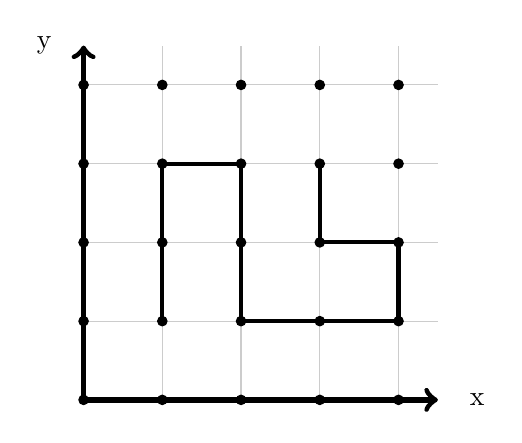
\begin{tikzpicture}

\node at ( 5,0) {x};
\node at (-0.5,4.5) {y};

\foreach \a in {0,...,4}{ 
	\draw[color=black!20!white] (\a,0)--(\a,4.5);
	\draw[color=black!20!white] (0,\a)--(4.5,\a);
 }

\draw[line width=2, ->] (0,0)--(4.5,0);
\draw[line width=2, ->] (0,0)--(0,4.5);

\foreach \a in {0,...,4}{
\foreach \x in {0,...,4}{
			\draw[fill=black] (\a,\x) circle (0.06);
	 }
}


\draw[line width=1.5] (1,1)--(1,2)--(1,3)--(2,3)--(2,1)--(4,1)--(4,2)--(3,2)--(3,3);
\end{tikzpicture} \\ 
Can we draw a curve that passes through all these points?  There are two strategies to try to hook around this many constraints:
\begin{itemize}
\item Lagrange Interpolation
\item Bezier Curves
\end{itemize} 
And maybe it depends on the type of constraint problem you are trying to solve: 
\begin{itemize}
\item passing through points
\item weaving arround points
\end{itemize}
I think one way to motivate a theory is to start with a problem you want to solve.\footnote{Other times, theories comes out of the box, complete. I think such theories are unusuable, or they leave from for input from you and me.  A comeback from that camp could be, ``John, why are you so obsessed with this particular problem?"  And I don't have any good reason.  Just because.  Sometimes about me, and the time and place makes me interested.  And I could be wrong!} We like to brag about how good we are at weaving around constraints.  How bad can we be?  Let $f: [0,1] \to \mathbb{R}$ be a real-valued function:
$$ f(x) = \left\{  \begin{array}{cc} 1 & x \notin \mathbb{Q}  \\ 
0 & x \in \mathbb{Q} \end{array} \right. $$
Then we can ask what the integral is between $0$ and $1$.  Overwhelmingly, the answer should be:
$$ \int_0^1 f(x) \, dx = 1 \times \Big|\{ x \notin \mathbb{Q}  \}\cap [0,1]\Big| + 0 \times \Big|\{ x \in \mathbb{Q}  \}\cap [0,1]\Big| =  1 $$
Relatively innocent-functions like these are sufficient Riemann integration.  I reasoned there are vastly more irrational numbers than rational numbers.


\newpage

\noindent This turns out to be one of the worse functions around, because it looks like $\mathbf{1}$ but isn't:
$$ f(x) \approx \mathbf{1} \quad\text{therefore}\quad \int f \approx \int \mathbf{1} $$
If I recall, we placed intervals around every single fraction $\frac{a}{b} \in \mathbb{Q}$ we get an upper estimate for how large this integral could be, and that upper estimate $ \to 0$.   \\ \\
How to deal with a function that often looks like $f(x) \equiv 1$ but isn't?\footnote{
One set of problems that plagued me was if we had two competing definition of  limit, maybe one returns a number and the other does not.  If we have two limiting procedures $1$ and $2$, maybe: 
$$ \big[ \lim \big]_1 \; a_n = A \quad\text{implies}\quad \big[ \lim \big]_2 \; a_n = A$$
Most of the time we don't really care how the limit procedure is defined.  Who cares really?
$$ N \gg 1 \quad \text{implies}\quad a_N \approx A$$
and the impliciation looks self-evident and most people won't question it.  The only reason we remember the exception is because that particular conversation went on record.} \\ 
\includegraphics{farey-01.png} \\
Here is a plot if we add all of the pure tones at all frequencies $\frac{a}{b}$ with $0 < a < b < 10$.  Theoretically we have found:
$$ \frac{1}{28} \sum_{0 < a < b < 10} e^{2\pi i \frac{a}{b} t} \approx \frac{1}{ c\, N^2 }  \sum_{0 < a < b < N} e^{2\pi i \frac{a}{b} t}
= \left\{ \begin{array}{cc}  1 & \text{if }t = 0 \\ 0 & \text{if }t \neq 0\end{array} \right.  $$
The constant in front is an oversimplification.  The odds of two numbers being relatively primes is a famous one:
$$ \phi(1) + \phi(2) + \dots + \phi(N) = \# \{ (a,b) : a < b \text{ and } \mathrm{gcd}(a,b)=1 \} \approx \frac{2}{\zeta(2)^2} $$
Analysis is the branch of math where we account for all the uses of the $\approx$  symbol.  What if I told you the function we just charted is $\approx {\color{blue}\mathbf{0}}$ ?

\newpage

\noindent When I read someone else's paper, a lot of my surprise stems from the author suggesting there is enough from in function space for something (very unlikely) to occur.  Let's make a little problem set: \\ \\
\# \textbf{1} Show constant function on the rational numbers integrates to zero:
$$ \int_{[0,1]} \mathbf{1}_{\mathbb{Q}} = 0 $$ 
\# \textbf{2} Find a curve that weaves around the obstacle course on page one:\\ \\
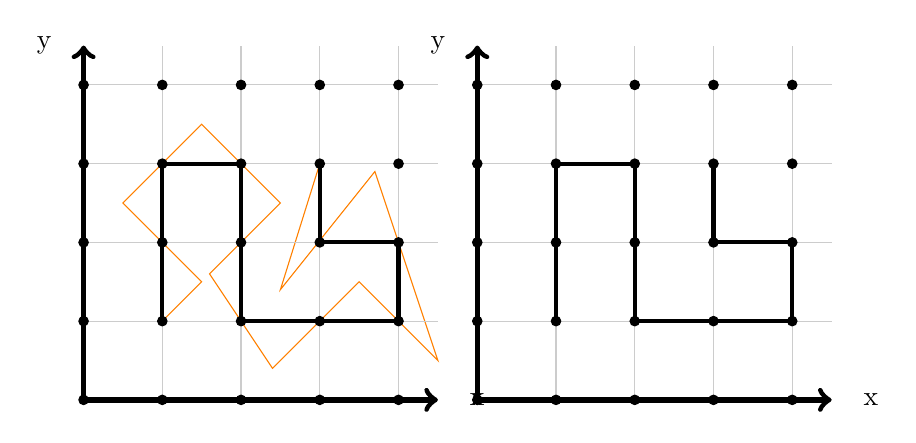
\begin{tikzpicture}

\begin{scope}

\node at ( 5,0) {x};
\node at (-0.5,4.5) {y};

\draw[color=red!50!yellow] (1, 1)--(1.5,1.5)--(0.5,2.5)--(1.5,3.5)--(2.5,2.5)--(1.6,1.6)--(2.4,0.4)
--(3.5,1.5)--(4.5,0.5)--(3.7,2.9)--(2.5,1.4)--(3,3);

\foreach \a in {0,...,4}{ 
	\draw[color=black!20!white] (\a,0)--(\a,4.5);
	\draw[color=black!20!white] (0,\a)--(4.5,\a);
 }

\draw[line width=2, ->] (0,0)--(4.5,0);
\draw[line width=2, ->] (0,0)--(0,4.5);

\foreach \a in {0,...,4}{
\foreach \x in {0,...,4}{
			\draw[fill=black] (\a,\x) circle (0.06);
	 }
}


\draw[line width=1.5] (1,1)--(1,2)--(1,3)--(2,3)--(2,1)--(4,1)--(4,2)--(3,2)--(3,3);



\end{scope}

\begin{scope}[xshift=5cm]

\node at ( 5,0) {x};
\node at (-0.5,4.5) {y};

\foreach \a in {0,...,4}{ 
	\draw[color=black!20!white] (\a,0)--(\a,4.5);
	\draw[color=black!20!white] (0,\a)--(4.5,\a);
 }

\draw[line width=2, ->] (0,0)--(4.5,0);
\draw[line width=2, ->] (0,0)--(0,4.5);

\foreach \a in {0,...,4}{
\foreach \x in {0,...,4}{
			\draw[fill=black] (\a,\x) circle (0.06);
	 }
}


\draw[line width=1.5] (1,1)--(1,2)--(1,3)--(2,3)--(2,1)--(4,1)--(4,2)--(3,2)--(3,3);

\end{scope}

\end{tikzpicture} 
With a pencil it's always possible to draw a curve that passes through all the dots.
Our challenge is to find an equation that passes through all the loops.  This is not so obvious it can always be done. \\ \\
\# \textbf{3} While I am remembering that my other example was going to be, we are going to solve the Prime Number Theorem.  
$$ \Lambda(n) = \left\{ \begin{array}{cl} \log p & \text{if }n=p \\ \\
0 & \text{not prime}\end{array} \right. $$
The prime number says that the density of primes is roughly $ \frac{1}{\text{\# digits}} $ it can also be phrased as:
$$ \sum_{n \leq x} \Lambda(n)  = x + o(x) $$
where $o(x)$ is a really small, unpredictible number\footnote{if you looked at my other projects, a great question to ask would be ``how small", and ``how unpredictible".  We could ask even though $o(x)$ is a small number, maybe it is bigger than $1$ or $5$ or $100$.} This won't be a review of number theory.  Just ironing out one or two parts in a previous discussion.  It's pretty hard. \\ \\
\# \textbf{4} Look at a real paper.  There are one or two short papers of Bourgain that I try to get through from time to time.\footnote{He does not write in a very forgiving way, and occasionally it's so bad, we may as well try to write the step ourselves.}
$$ f(t) = \sum_{|x|, |y|, |z| < N} e^{2\pi i t \; (x^2 + y^2 - \sqrt{2} z^2)} $$ 
This is my favorite way to cause trouble and I get the sense this is the recommended way to start.  A sense that comes from nowhere. .
 \\ \\

\newpage

\noindent All good project start from raw ingredients and tell a story.\footnote{On day I got a textbook ``Methods in Mathematical Physics (Vol 1)"  The book is in German so maybe that's why it was so cheap; it is available in English.  These math-for-phyisicists textbooks are pretty dull.  This is the middle of the 20th century and Math and Physics, which you'd assume were related had taken very different paths.  Mathematicians were tired of calculations and instead proposed to build a world entirely of abstrct principles.  Physicists needed to build things and used math whenever they needed it, or fabricated their own\dots Courant-Hilbert managed to write a textbook that assembles hundreds of unrelated techniques into a pretty-good story.  And it's still the story in the modern literature, more or less.}  For me pictures form an engine that start projects.  Or it could be a memory or something that happened. \\
\includegraphics[width=5in]{node-01.png} \\ 
These pictures of the vibrating nodes (``notes" \quarternote\twonotes\quarternote\, ) of a square drum were made are before computer graphics (the textbook was written in the 1930s). Drafting and technical drawing (without computers) seems like stupid and arcane technical skill, but our ability to make things of good quality is constrained by this.  Maybe the textbooks fail to make the case. \\
\includegraphics[width=5in]{node-02.png} \\ 
Generating these curves with computer is not so easy.  The equation for both of these is:
$$ f(x,y) = 0 $$
for some judiciously chosen function $f$.  In the case of the square we can try sines and cosines:
$$ f(x,y) = \sum_{m, n \in \mathbb{Z}} a_{m,n} \sin m x \sin n y$$
Maybe I need to include cosines as well.  Different variations.  Why stop at two?  Maybe I can get \textit{every possible pattern} using a level-set of bunch of sine and cosine. \\ \\Additionally, even when we have the equation, solving $f(x,y) = 0$ is not very realistic, maybe solving $f(x,y) < \epsilon$ where $\epsilon =  10^{-3}$ or $10^{-6}$ or however small you are intereted in.  And this becomes an algorithms problem. \\ \\
In the process I may have mixed up two kinds of problems:
\begin{itemize}
\item Drawing the curve (maybe with Bezier curves)
\item Finding a function with reasonable level set (maybe with Lagrange Interpolation)
\end{itemize}
I think they're almost the same but after reading Wikipedia I might be wrong.  When I started off in number theory, there are all these cute averaging statements, such as:
$$  \frac{1}{r_3(n)}\sum_{x^2 + y^2 + z^2 = n} \phi(x,y,z) \ll n^{-1/28} $$
All of these theorems rest on the interpolation results I'm trying to explore here\dots and perhaps all of these number theory problems are sources of ill-behaved functions I am outlining.  \\ \\
All the papers I have seen resort to horrible complicated rearrangements that deserve a better explanation.  

\newpage

\noindent \# \textbf{1} Starting small, let's show that $ \int \mathbf{1}_\mathbb{Q} = 0 $.  The rational numbers are dense but form a set of measure zero.
\begin{itemize}
\item $\overline{\mathbb{Q}}= \mathbb{R}$
\item $\mu(\mathbb{Q}) = 0$
\end{itemize}
You could take for granted that you can always find a fraction close enough to your number 
$$ 47\% = \frac{47}{100} \approx \frac{12}{25} $$
\textbf{12 in 25} sounds pretty good instead of \textbf{47 in 100}.  Maybe one is more persuasive than the other.\footnote{Here we use a tiny bit of projective space $\frac{a}{b} = [a:b] = \mathbb{Q}P^1$ and maybe even a tiny bit of the Galois cohomology of the field $\mathbb{Q}$.  That is my theory what all these $H^1$'s are doing there. }  Even though we say $\mathbb{Q}$ is dense in $\mathbb{R}$, finding any fraction is easy, finding a really good fraction can be some work.  If $\alpha \notin \mathbb{Q}$: 
$$ \exists \, p,q \text{ such that }  \bigg| \frac{p}{q} - \alpha \bigg| < \frac{1}{q^2} $$
Therefore density misses other more refined statements we could make about $\overline{\mathbb{Q}}$. \\ \\
Let's walk through a few sample arguments.\footnote{At my school, real analysis at the level of Lebesgue Theory was taught to 3rd year undergraduates who were pretty serious about math. I failed it.  And passed the second time with a B.  These days I almost agree with their assessment because I look at the textbook and still don't really get it.}  I can't look at this picture and not see Dehn's theorem, that if the length and the width are rational, then every single rectangle must have rational length and width.\\ 
\includegraphics[width=3in]{stein-01.png}
\includegraphics[width=4.5in]{stein-02.png} \\ 
I could have spent an entire semester drawing ever more complicated shapes and putting rectangles on them. \\
 \\

\newpage

\vfill


\noindent 

\begin{thebibliography}{}

\item Richard Courant, David Hilbert.  \textbf{Methoden der mathematischen Physik} (Satz I) Springer, 1937. 

\item Elias Stein, Rami Shakarchi.   \textbf{Analysis III: Real Analysis - Measure Theory, Integration and Hilbert Space }(Princeton Lectures in Analysis) Princeton University Press, 2004.


\end{thebibliography}

\vfill

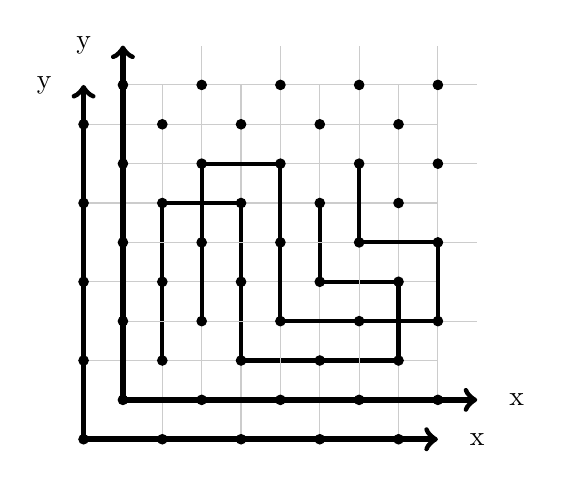
\begin{tikzpicture}

\node at ( 5,0) {x};
\node at (-0.5,4.5) {y};

\foreach \a in {0,...,4}{ 
	\draw[color=black!20!white] (\a,0)--(\a,4.5);
	\draw[color=black!20!white] (0,\a)--(4.5,\a);
 }

\draw[line width=2, ->] (0,0)--(4.5,0);
\draw[line width=2, ->] (0,0)--(0,4.5);

\foreach \a in {0,...,4}{
\foreach \x in {0,...,4}{
			\draw[fill=black] (\a,\x) circle (0.06);
	 }
}


\draw[line width=1.5] (1,1)--(1,2)--(1,3)--(2,3)--(2,1)--(4,1)--(4,2)--(3,2)--(3,3);


\begin{scope}[xshift=0.5cm, yshift=0.5cm]

\node at ( 5,0) {x};
\node at (-0.5,4.5) {y};

\foreach \a in {0,...,4}{ 
	\draw[color=black!20!white] (\a,0)--(\a,4.5);
	\draw[color=black!20!white] (0,\a)--(4.5,\a);
 }

\draw[line width=2, ->] (0,0)--(4.5,0);
\draw[line width=2, ->] (0,0)--(0,4.5);

\foreach \a in {0,...,4}{
\foreach \x in {0,...,4}{
			\draw[fill=black] (\a,\x) circle (0.06);
	 }
}


\draw[line width=1.5] (1,1)--(1,2)--(1,3)--(2,3)--(2,1)--(4,1)--(4,2)--(3,2)--(3,3);
\end{scope}


\end{tikzpicture}



\end{document}